% file: sections/dfs-bfs.tex

%%%%%%%%%%%%%%%%%%%%
\begin{frame}{}
  \begin{columns}
	\column{0.50\textwidth}
	  \fignocaption{width = 0.40\textwidth}{figs/hopcroft.jpg}{\centerline{John Hopcroft}}
	\column{0.50\textwidth}
	  \fignocaption{width = 0.35\textwidth}{figs/tarjan.png}{\centerline{Robert Tarjan}}
  \end{columns}

  \vspace{0.50cm}
  \begin{quote}
    \textcolor{blue}{``For fundamental achievements in the design and analysis of algorithms and data structures.''} \\
    \hfill --- Turing Award, 1986
  \end{quote}
\end{frame}
%%%%%%%%%%%%%%%%%%%%
\begin{frame}{Depth-first search}
  \fignocaption{width = 0.55\textwidth}{figs/dfs-paper-tarjan}

  \uncover<2->{
    \begin{quote}
      {\small ``We \textcolor{red}{have seen} how the depth-first search method may be used in the construction of
      very efficient graph algorithms. $\dots$ \\
      Depth-first search \textcolor{red}{is} a powerful technique with many applications.''}
    \end{quote}
  }

  \begin{alertblock}{Reference}
    \begin{itemize}
      \item ``Depth-First Search And Linear Graph Algorithms'' by Robert Tarjan.
    \end{itemize}
  \end{alertblock}
\end{frame}
%%%%%%%%%%%%%%%%%%%%
\begin{frame}{The POWER of DFS} 
  \begin{center}
	Graph decomposition vs. Graph traversal \\[10pt]
	Structures!
  \end{center}

  \pause
  \begin{enumerate}
	\item states of vertices
	\item types of edges
	\item lifetime of vertices (DFS)
	  \begin{itemize}
	    \item $v: \text{d}[v], \text{f}[v]$
	    \item $\text{f}[v]$: DAG, SCC
	    \item $\text{d}[v]$: biconnectivity
	  \end{itemize}
  \end{enumerate}
\end{frame}
%%%%%%%%%%%%%%%%%%%%
\begin{frame}{Types of edges}
  \begin{definition}[Classifying edges]
    Given a DFS/BFS traversal $\Rightarrow$ DFS/BFS tree:
	\begin{description}[Forward edge:]
	  \item[Tree edge:] $\to$ child
	  \item[Back edge:] $\to$ ancestor
	  \item[Forward edge:] $\to$ \emph{nonchild} descendant
	  \item[Cross edge:] $\to$ neither ancestor nor descendant
    \end{description}
  \end{definition}

  \pause
  \begin{alertblock}{Remarks}
    \begin{itemize}
      \item applicable to both DFS and BFS
      \item w.r.t. DFS/BFS trees
    \end{itemize}
  \end{alertblock}
\end{frame}
%%%%%%%%%%%%%%%%%%%%

%%%%%%%%%%%%%%%%%%%%
\begin{frame}{}
  \begin{columns}
    \column{0.50\textwidth}
      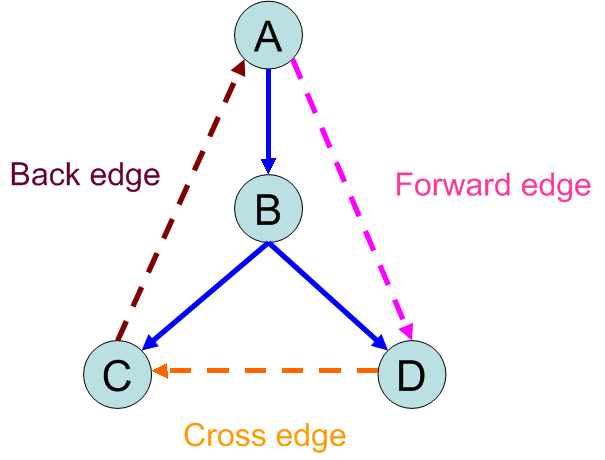
\includegraphics[width = 0.80\textwidth]{figs/dfs-digraph.png}

      \vspace{0.50cm}
      \centerline{\purple{DFS on directed graph}}
    \pause
    \column{0.50\textwidth}
      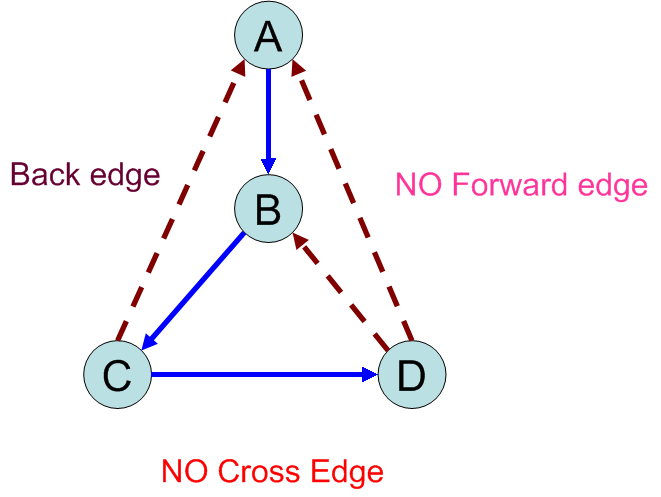
\includegraphics[width = 0.80\textwidth]{figs/dfs-undirected.png}

      \vspace{0.50cm}
      \centerline{\purple{DFS on undirected graph}}
  \end{columns}
\end{frame}
%%%%%%%%%%%%%%%%%%%%

%%%%%%%%%%%%%%%%%%%%
\begin{frame}{}
  \begin{columns}
    \column{0.50\textwidth}
      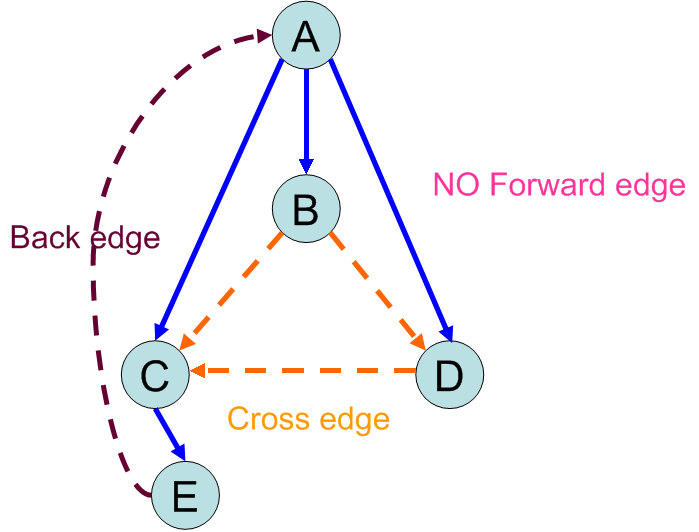
\includegraphics[width = 0.80\textwidth]{figs/bfs-digraph.png}

      \vspace{0.50cm}
      \centerline{\purple{BFS on directed graph}}
    \pause
    \column{0.50\textwidth}
      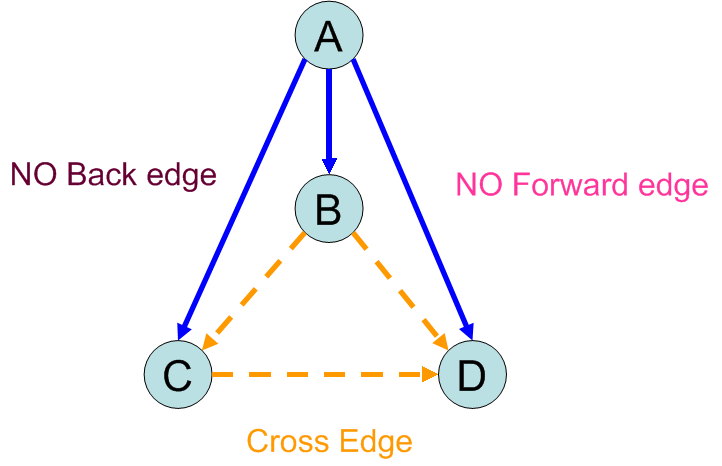
\includegraphics[width = 0.95\textwidth]{figs/bfs-undirected.png}

      \vspace{0.50cm}
      \centerline{\purple{BFS on undirected graph}}
  \end{columns}
\end{frame}
%%%%%%%%%%%%%%%%%%%%

%%%%%%%%%%%%%%%%%%%%
\begin{frame}{}
  \begin{exampleblock}{DFS tree and BFS tree coincide (Problem $5.7$)}
    \centerline{Undirected connected graph $G = (V,E), v \in V$}
      
    \[
      \text{DFS tree } T \text{ from } v \equiv \text{ BFS tree } T' \text{ from } v
    \]

    \pause
    \[
      \red{G \equiv T}
    \]
  \end{exampleblock}

  \pause
  \vspace{0.30cm}
  \begin{proof}
    \centerline{$G_{\text{DFS}}$: tree + back \emph{vs.} $G_{\text{BFS}}$: tree + cross}
  \end{proof}

  \pause
  \vspace{0.30cm}
  \begin{center}
    \red{$Q:$} What if $G$ is a digraph?
  \end{center}
\end{frame}
%%%%%%%%%%%%%%%%%%%%
\begin{frame}{}
  \centerline{\red{\Large Lift time of vertices in DFS}}
  \fignocaption{width = 0.45\textwidth}{figs/active-interval.png}
\end{frame}
%%%%%%%%%%%%%%%%%%%%
\begin{frame}{}
  \begin{theorem}[Disjoint or Contained (Problem $4.2$: (1) \& (2))]
    \[
      \forall u,v: [_{u} \; ]_{u} \cap [_{v} \; ]_{v} = \emptyset \bigvee 
      \Big([_{u} \; ]_{u} \subsetneqq [_{v} \; ]_{v} \lor [_{v} \; ]_{v} \subsetneqq [_{u} \; ]_{u}\Big)
    \]
  \end{theorem}

  \pause

  \begin{proof}
	\fignocaption{width = 0.30\textwidth}{figs/stack.png}
  \end{proof}
\end{frame}
%%%%%%%%%%%%%%%%%%%%
\begin{frame}{}
  \begin{exampleblock}{Preprocessing for \red{ancestor/descendant} relation (Problem 5.23)}
    \fignocaption{width = 0.45\textwidth}{figs/binary-tree}

    \centerline{\red{\large $Q:$ \it Is $u$ an ancestor of $v$? $O(1)$}}
  \end{exampleblock}

  \pause
  \[
    v: \text{d}[v], \text{f}[v]
  \]

  \pause
  \vspace{-0.20cm}
  \[
    \red{Q: } \text{ \# of descendants of any } v?
  \]
\end{frame}
%%%%%%%%%%%%%%%%%%%%
\begin{frame}{}
  \begin{exampleblock}{Edge types and life time of vertices in DFS (Problem $4.5$)}
    \[
      \forall u \to v:
    \]
    \vspace{-0.30cm}
    \begin{itemize}
      \item tree/forward edge: $\red{[_{u}}\; \teal{[_{v}\; ]_{v}}\; \red{]_{u}}$
      \item back edge: $\teal{[_{v}}\; \red{[_{u}\; ]_{u}}\; \teal{]_{v}}$
      \item cross edge: $\teal{[_{v}\; ]_{v}}\; \red{[_{u}\; ]_{u}}$
    \end{itemize}
  \end{exampleblock}

  \pause
  \[
    \text{f}[v] < \text{d}[u] \iff \text{ \uncover<3->{\brown{cross}} edge}
  \]


  \[
    \uncover<4->{\text{f}[u] < \text{f}[v] \iff } \uncover<5->{\text{ \red{back} edge }}
  \]
  \[
    \nexists \text{ cycle} \implies \uncover<6->{\red{\boxed{u \to v \iff \text{f}[v] < \text{f}[u]}}}
  \]
\end{frame}
%%%%%%%%%%%%%%%%%%%%
\begin{frame}{}
  \begin{exampleblock}{Height and diameter of tree (Problem $5.4$)}
    Binary tree $T = (V, E)$ with $|V| = n$:
    \begin{itemize}
      \item height $H(T)$ in $O(n)$
      \item diameter $D(T)$ in $O(n)$
    \end{itemize}
  \end{exampleblock}

  \pause
  \vspace{0.30cm}
  \[
    \left\{\begin{array}{ll}
      H(T) = 0, & T \text{ is a leave} \\
      H(T) = \max\Big(H(L_T), H(R_T)\Big) + 1, & \text{o.w.}
    \end{array}\right.
  \]
  \centerline{throught root or not?}

  \pause
  \vspace{0.50cm}
  \begin{alertblock}{Question}
	Diameter of a tree \emph{without} a designated root?
  \end{alertblock}
\end{frame}
%%%%%%%%%%%%%%%%%%%%
\begin{frame}{Perfect subtree}
  \begin{exampleblock}{Perfect subtree (Problem 5.22)}
	\begin{itemize}
	  \item binary tree $T = (V, E)$
	  \item root $r \in V$
	  \item goal: find all perfect subtrees
	\end{itemize}
  \end{exampleblock}
\end{frame}
%%%%%%%%%%%%%%%%%%%%
\begin{frame}{Counting shortest paths}
  \begin{exampleblock}{Counting shortest paths (Problem 5.26)}
	Counting \# of shortest paths in (un)directed graphs using BFS.
  \end{exampleblock}

  \pause
  \vspace{0.50cm}
  \centerline{Maybe in the next class$\dots$}
\end{frame}
%%%%%%%%%%%%%%%%%%%%
